% Slides for hello-analyser.tex: its diagrams, under its headings.
% Build with ./build.sh hello-analyser-slides.tex (latexmk; settings in .latexmkrc).

\documentclass[aspectratio=169,11pt]{beamer}

\usepackage{deck}

\begin{document}

\begin{frame}{\huge Hello world on the logic analyser}
  \begin{fig}
  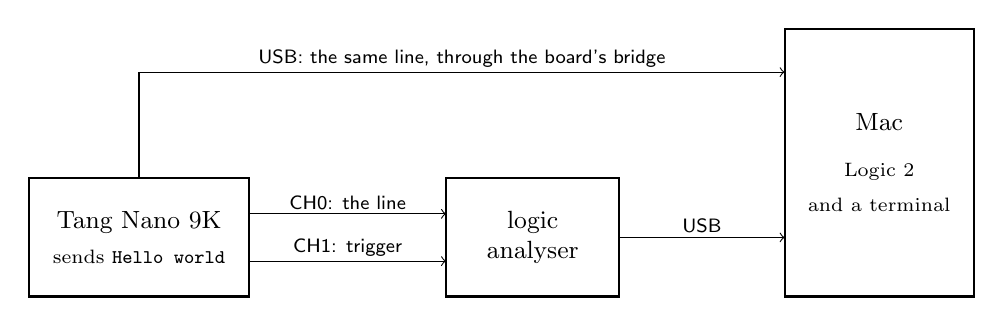
\begin{tikzpicture}[box/.style={draw, thick, align=center, font=\small},
      wire/.style={->}, lbl/.style={font=\scriptsize\sffamily, above, inner sep=1.5pt}]
    \node[box, minimum width=2.8cm, minimum height=1.5cm] (fpga) at (0,0) {\name{Tang Nano 9K}\\[0.2em]\scriptsize sends \texttt{Hello world}};
    \node[box, minimum width=2.2cm, minimum height=1.5cm] (la) at (5,0) {logic\\analyser};
    \node[box, minimum width=2.4cm, minimum height=3.4cm] (mac) at (9.4,0.95) {Mac\\[0.6em]\scriptsize Logic~2\\[0.2em]\scriptsize and a terminal};
    \draw[wire] (1.4,0.3) -- node[lbl] {CH0: the line} (3.9,0.3);
    \draw[wire] (1.4,-0.3) -- node[lbl] {CH1: trigger} (3.9,-0.3);
    \draw[wire] (6.1,0) -- node[lbl] {USB} (8.2,0);
    \draw[wire] (0,0.75) |- node[lbl, pos=0.75] {USB: the same line, through the board’s bridge} (8.2,2.1);
  \end{tikzpicture}
  \end{fig}
\end{frame}

\begin{frame}{Wiring}
  \begin{fig}
  \vmid{\begin{tikzpicture}[
      port/.style={font=\footnotesize\ttfamily},
      pin/.style={font=\scriptsize, above, inner sep=1.5pt},
      blk/.style={draw, thick, align=center, font=\small, minimum height=0.9cm},
      hdr/.style={draw, fill=white, circle, inner sep=1.6pt},
      title/.style={font=\small\bfseries, inner sep=3pt}]
    % the development board, and the FPGA on it
    \draw[black!45, rounded corners=3pt] (-3.6,-2.5) rectangle (5.6,2.7);
    \node[title, anchor=south west] at (-3.6,-2.5) {\name{Tang Nano 9K}};
    \draw[thick] (-1.8,-1.7) rectangle (1.8,2.2);
    \node[title, anchor=north] at (0,2.2) {\name{GW1NR-9}};
    \node[port, anchor=west] at (-1.75,0) {sys\_clk};
    \node[port, anchor=east] at (1.75,1.5) {tx};
    \node[port, anchor=east] at (1.75,-0.2) {tx\_probe};
    \node[port, anchor=east] at (1.75,-1.0) {busy};
    % the 27 MHz crystal, and the FPGA pin numbers where each wire leaves the chip
    \pic at (-2.9,0) {crystal};
    \node[font=\scriptsize, below] at (-2.9,-0.4) {27\,MHz};
    \draw[->] (-2.6,0) -- (-1.8,0);
    \node[pin] at (-2.1,0) {52};
    \node[blk, anchor=west] (usb) at (2.7,1.5) {\name{BL702}\\[-0.1em]\scriptsize USB-serial bridge};
    \draw[->] (1.8,1.5) -- (usb);
    \node[pin] at (2.1,1.5) {17};
    \draw[->] (1.8,-0.2) -- (6.5,-0.2);
    \node[pin] at (2.1,-0.2) {31};
    \draw[->] (1.8,-1.0) -- (6.5,-1.0);
    \node[pin] at (2.1,-1.0) {32};
    \draw (5.6,-1.8) -- (6.5,-1.8);
    % header pins on the board's edge, named as in the board figure
    \foreach \y/\l in {-0.2/R21, -1.0/R22, -1.8/R23} {
      \node[hdr] at (5.6,\y) {};
      \node[pin, anchor=south west] at (5.7,\y) {\name{\l}};
    }
    % off the board: the Mac above the analyser
    \node[blk, minimum width=2.0cm] (mac) at (7.5,1.5) {Mac\\terminal};
    \draw[->] (usb) -- node[font=\scriptsize\itshape, above, pos=0.55] {USB} (mac);
    \draw[thick] (6.5,-2.2) rectangle (8.5,0.55);
    \node[font=\small, anchor=north, align=center, inner sep=2pt] at (7.5,0.55) {analyser};
    \node[font=\footnotesize, anchor=west] at (6.6,-0.2) {\name{CH0}};
    \node[font=\footnotesize, anchor=west] at (6.6,-1.0) {\name{CH1}};
    \node[font=\footnotesize, anchor=west] at (6.6,-1.8) {\name{GND}};
  \end{tikzpicture}}\quad
  \vmid{\boardpins{r/21/R21/-1, r/22/R22/0, r/23/R23/1}}
  \end{fig}
\end{frame}

\begin{frame}{One message, then rest}
  \begin{fig}
  \begin{tikztimingtable}[timing/slope=0.1, xscale=1.35, yscale=1.4, timing/name/.style={font=\small\ttfamily},
      timing/d/text/.style={font=\scriptsize\ttfamily}]
    busy & L 13H 4L H \\
    tx   & H D{H}D{e}D{l}D{l}D{o}D{\textvisiblespace}D{w}D{o}D{r}D{l}D{d}D{\textbackslash r}D{\textbackslash n} 4H D{H} \\
  \extracode
    \foreach \y in {0.5,-1.5} \node[fill=white, inner sep=1pt, font=\small] at (16,\y) {//};
    \draw[<->] (1.05,-3.3) -- node[below, font=\scriptsize] {1.13\,ms: 13 frames} (14.05,-3.3);
    \draw[<->] (14.05,-3.3) -- node[below, font=\scriptsize] {100\,ms} (18.05,-3.3);
  \end{tikztimingtable}
  \end{fig}
\end{frame}

\begin{frame}{One character: a frame}
  \begin{fig}
  \begin{tikztimingtable}[timing/slope=0.1, xscale=2.2, yscale=1.5, timing/name/.style={font=\small\ttfamily}]
    tx & H L L L L H L L H L H H \\
  \extracode
    \vertlines[black!20]{1.05,2.05,...,11.05}  % through each edge's midpoint: the slope is 0.1
    \foreach \l [count=\i from 0] in {rest, start, 0, 0, 0, 1, 0, 0, 1, 0, stop, rest}
      \node[font=\scriptsize] at (\i+0.55,-1.4) {\l};
  \end{tikztimingtable}
  \end{fig}
\end{frame}

\begin{frame}{The state machine}
  \begin{fig}
  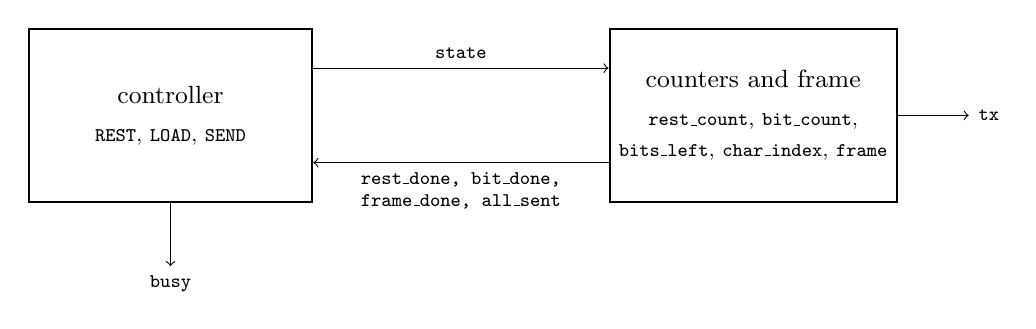
\begin{tikzpicture}[blk/.style={draw, thick, align=center, font=\small, minimum width=3.6cm, minimum height=2.2cm},
      sig/.style={font=\scriptsize\ttfamily, align=center}]
    \node[blk] (ctl) at (0,0) {controller\\[0.3em]\scriptsize\texttt{REST}, \texttt{LOAD}, \texttt{SEND}};
    \node[blk] (cnt) at (7.4,0) {counters and frame\\[0.3em]\scriptsize\texttt{rest\_count}, \texttt{bit\_count},\\\scriptsize\texttt{bits\_left}, \texttt{char\_index}, \texttt{frame}};
    \draw[->] ([yshift=0.6cm]ctl.east) -- node[sig, above] {state} ([yshift=0.6cm]cnt.west);
    \draw[->] ([yshift=-0.6cm]cnt.west) -- node[sig, below] {rest\_done, bit\_done,\\ frame\_done, all\_sent} ([yshift=-0.6cm]ctl.east);
    \draw[->] (ctl.south) -- ++(0,-0.8) node[sig, below] {busy};
    \draw[->] (cnt.east) -- ++(0.9,0) node[sig, right] {tx};
  \end{tikzpicture}
  \end{fig}
\end{frame}

\begin{frame}{The controller}
  \begin{fig}
  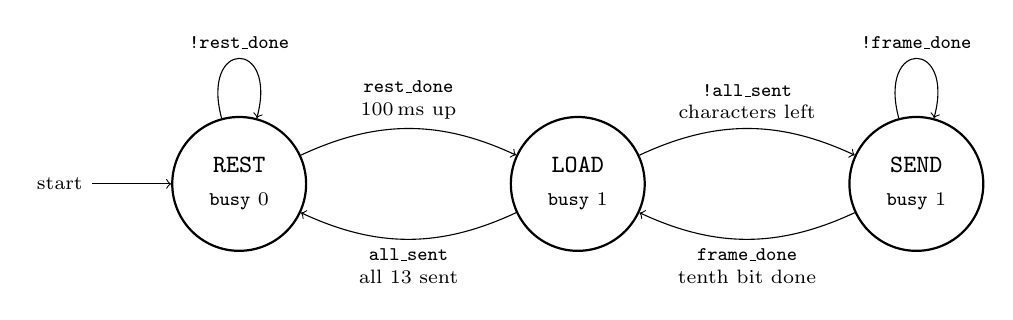
\begin{tikzpicture}[st/.style={draw, thick, circle, minimum size=1.7cm, align=center, font=\small},
      lbl/.style={font=\scriptsize, align=center}]
    \node[st] (rest) at (0,0) {\texttt{REST}\\[0.1em]\scriptsize \texttt{busy} 0};
    \node[st] (load) at (4.3,0) {\texttt{LOAD}\\[0.1em]\scriptsize \texttt{busy} 1};
    \node[st] (send) at (8.6,0) {\texttt{SEND}\\[0.1em]\scriptsize \texttt{busy} 1};
    \draw[->] (rest) to[bend left=25] node[lbl, above] {\texttt{rest\_done}\\ 100\,ms up} (load);
    \draw[->] (load) to[bend left=25] node[lbl, above] {\texttt{!all\_sent}\\ characters left} (send);
    \draw[->] (send) to[bend left=25] node[lbl, below] {\texttt{frame\_done}\\ tenth bit done} (load);
    \draw[->] (load) to[bend left=25] node[lbl, below] {\texttt{all\_sent}\\ all 13 sent} (rest);
    \draw[->] (rest) to[loop above, looseness=6] node[lbl, above] {\texttt{!rest\_done}} (rest);
    \draw[->] (send) to[loop above, looseness=6] node[lbl, above] {\texttt{!frame\_done}} (send);
    \draw[<-] (rest.west) -- ++(-1,0) node[left, lbl] {start};
  \end{tikzpicture}
  \end{fig}
\end{frame}

\begin{frame}{In simulation}
  \begin{fig}
  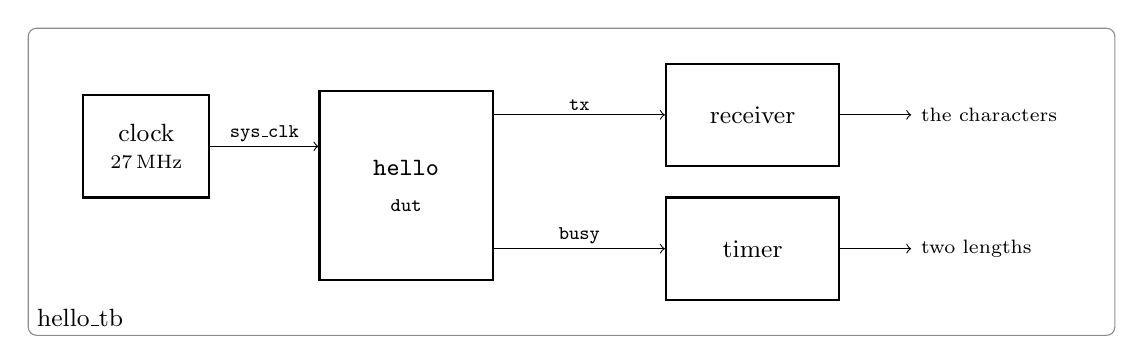
\begin{tikzpicture}[blk/.style={draw, thick, align=center, font=\small, minimum height=1.3cm},
      sig/.style={font=\scriptsize\ttfamily, above, inner sep=1.5pt}]
    \draw[black!45, rounded corners=3pt] (-1.2,-2.4) rectangle (12.6,1.5);
    \node[font=\small, anchor=south west, inner sep=3pt] at (-1.2,-2.4) {\name{hello\_tb}};
    \node[blk, minimum width=1.6cm] (clk) at (0.3,0) {clock\\[-0.1em]\scriptsize 27\,MHz};
    \node[blk, minimum width=2.2cm, minimum height=2.4cm] (dut) at (3.6,-0.5) {\texttt{hello}\\[0.2em]\scriptsize \texttt{dut}};
    \node[blk, minimum width=2.2cm] (rx) at (8.0,0.4) {receiver};
    \node[blk, minimum width=2.2cm] (tm) at (8.0,-1.3) {timer};
    \draw[->] (clk) -- node[sig] {sys\_clk} (clk -| dut.west);
    \draw[->] (dut.east |- rx) -- node[sig] {tx} (rx);
    \draw[->] (dut.east |- tm) -- node[sig] {busy} (tm);
    \draw[->] (rx.east) -- ++(0.9,0) node[right, font=\scriptsize] {the characters};
    \draw[->] (tm.east) -- ++(0.9,0) node[right, font=\scriptsize] {two lengths};
  \end{tikzpicture}
  \end{fig}
\end{frame}

\begin{frame}{How the receiver reads a frame}
  \begin{fig}
  \begin{tikztimingtable}[timing/slope=0.1, xscale=3.2, yscale=1.5, timing/name/.style={font=\small\ttfamily}]
    tx & H L L L L H L L H L H H \\
  \extracode
    \vertlines[black!20]{1.05,2.05,...,11.05}
    \foreach \l [count=\i from 0] in {rest, start, 0, 0, 0, 1, 0, 0, 1, 0, stop, rest}
      \node[font=\scriptsize] at (\i+0.55,-1.4) {\l};
    \foreach \x in {2.55,3.55,...,10.55} \draw[->, thick] (\x,2.0) -- (\x,1.05);
    \draw[<->] (1.05,-2.3) node[left, font=\scriptsize] {½ bit} -- (1.55,-2.3);
    \draw[<->] (1.55,-2.3) -- node[below, font=\scriptsize] {1 bit} (2.55,-2.3);
  \end{tikztimingtable}
  \end{fig}
\end{frame}

\end{document}
